\setauthor{\firstauthor}
\subsection{Fragenkonfigurator}
\begin{figure}[h t]
    \centering
    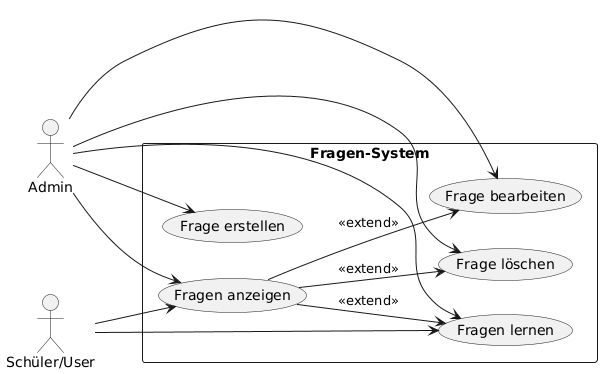
\includegraphics[width=0.6\textwidth]{pics/fragenkonf_usecase.png}
    \caption{Usecases Fragenkonfigurator}
\end{figure}

Das Fragen-System der Matura-Vorbereitungsplattform ermöglicht den Nutzern, gezielt Fragen zu erstellen, zu verwalten und zum Lernen zu verwenden. Dabei unterscheiden sich die Rechte der Akteure deutlich:

\subsubsection{Admin-Rechte}
\begin{itemize}
    \item Der Admin kann neue Fragen erstellen, bestehende Fragen bearbeiten und Fragen löschen. Dadurch behält er die Kontrolle über die Qualität und Relevanz der Lerninhalte.
    \item Der Admin kann alle Fragen einsehen und für den Lernprozess nutzen. So kann er die Plattform sowohl zur Verwaltung als auch zur eigenen Vorbereitung verwenden.
\end{itemize}

\subsubsection{Schüler-/User-Rechte}
\begin{itemize}
    \item Schüler haben eingeschränkte Rechte und können Fragen nur anzeigen und lernen. 
    \item Sie können keine Fragen bearbeiten oder löschen, wodurch die Integrität des Fragenpools erhalten bleibt.
    \item Der Lernprozess erfolgt ohne Rückmeldung über richtige oder falsche Antworten, um eine einfache und stressfreie Wiederholung zu ermöglichen.
\end{itemize}

\subsubsection{Funktionale Übersicht}
\begin{itemize}
    \item \textbf{Fragen erstellen:} Nur Admins können neue Fragen anlegen.
    \item \textbf{Fragen bearbeiten/löschen:} Admins können bestehende Fragen ändern oder entfernen.
    \item \textbf{Fragen anzeigen:} Alle Nutzer können Fragen einsehen.
    \item \textbf{Fragen lernen:} Alle Nutzer können die Fragen durchgehen, ohne dass das System Feedback gibt.
\end{itemize}